\documentclass{article}

\usepackage{amsmath}
\usepackage{tabularx}
\usepackage[table]{xcolor}
\usepackage{hyperref}
\usepackage{cleveref}
\usepackage{tikz}
\usetikzlibrary{positioning, calc, shapes, arrows, fit}
\usepackage{circuitikz}
\usepackage{subcaption}
\usepackage[colorinlistoftodos]{todonotes}
\linespread{0.9}
\hypersetup{
    colorlinks = true,
    linkbordercolor = {black}
}
\begin{document}
\title{Lab 2 -- Using the Si5351 clock generator circuit with ItsyBitsy}
\author{
    Yifan Zhu\\
    Lab Partner: John Kustin
}
\maketitle

\begin{abstract}
    We use an ItsyBitsy to build a Si5352 clock generator circuit to generate waveforms at various frequencies.
\end{abstract}

\section{Introduction}
In various circuits we need ``clock signals'' at some precise frequency.
A modern solution is to use clock generator ICs, which have advantages of being low-cost, having reasonable performance, and being able to generate signals at different frequencies with a single IC.

In this lab we will generate clock signals using the
\href{https://cdn-shop.adafruit.com/datasheets/Si5351.pdf}{Si5351} IC,
and we will send the control $\text{I}^2\text{C}$ signals to the Si5351 using the \href{https://learn.adafruit.com/introducing-adafruit-itsybitsy-m4}{ItsyBitsy} microcontroller and CircuitPython.

\section{Experimental Setup}

We did the assembly following the instructions \href{https://learn.adafruit.com/adafruit-si5351-clock-generator-breakout/overview}{online at adafruit}, while replacing the pinout for the Arduino microcontroller with that of the ItsyBitsy microcontroller:

\begin{enumerate}
    \item We soldered pins onto the ItsyBitsy and the Si5351 breakout board.
    \item We soldered SMA connectors onto the Si5351 breakout board.
          SMA connectors are needed to carry the generated clock signals that are essentially RF.
    \item According to the documentation of \href{https://learn.adafruit.com/adafruit-si5351-clock-generator-breakout/pinouts}{Adafruit Si5351 Breakout Board} and \href{https://cdn-learn.adafruit.com/downloads/pdf/introducing-adafruit-itsybitsy-m4.pdf}{ItsyBitsy}, using jumper wires we connected
          \begin{enumerate}
              \item the 3V pin (ItsyBitsy) to the Vin pin (Si5351 breakout),
              \item the GND pin (ItsyBitsy) to the GND pin (Si5351 breakout),
              \item the SCL pin (ItsyBitsy) to the SCL pin (Si5351 breakout),
              \item and the SDA pin (ItsyBitsy) to the SDA pin (Si5351 breakout).
          \end{enumerate}
    \item We updated the bootloader of the ItsyBitsy following the \href{https://learn.adafruit.com/introducing-adafruit-itsybitsy-m4/update-the-uf2-bootloader}{instructions}.
          And we installed CircuitPython following the instructions \href{https://learn.adafruit.com/introducing-adafruit-itsybitsy-m4/circuitpython}{here}.
    \item And the CircuitPython code is taken directly from the \href{https://learn.adafruit.com/adafruit-si5351-clock-generator-breakout/circuitpython}{Adafruit website}.
\end{enumerate}

\begin{figure}[h]
    \centering
    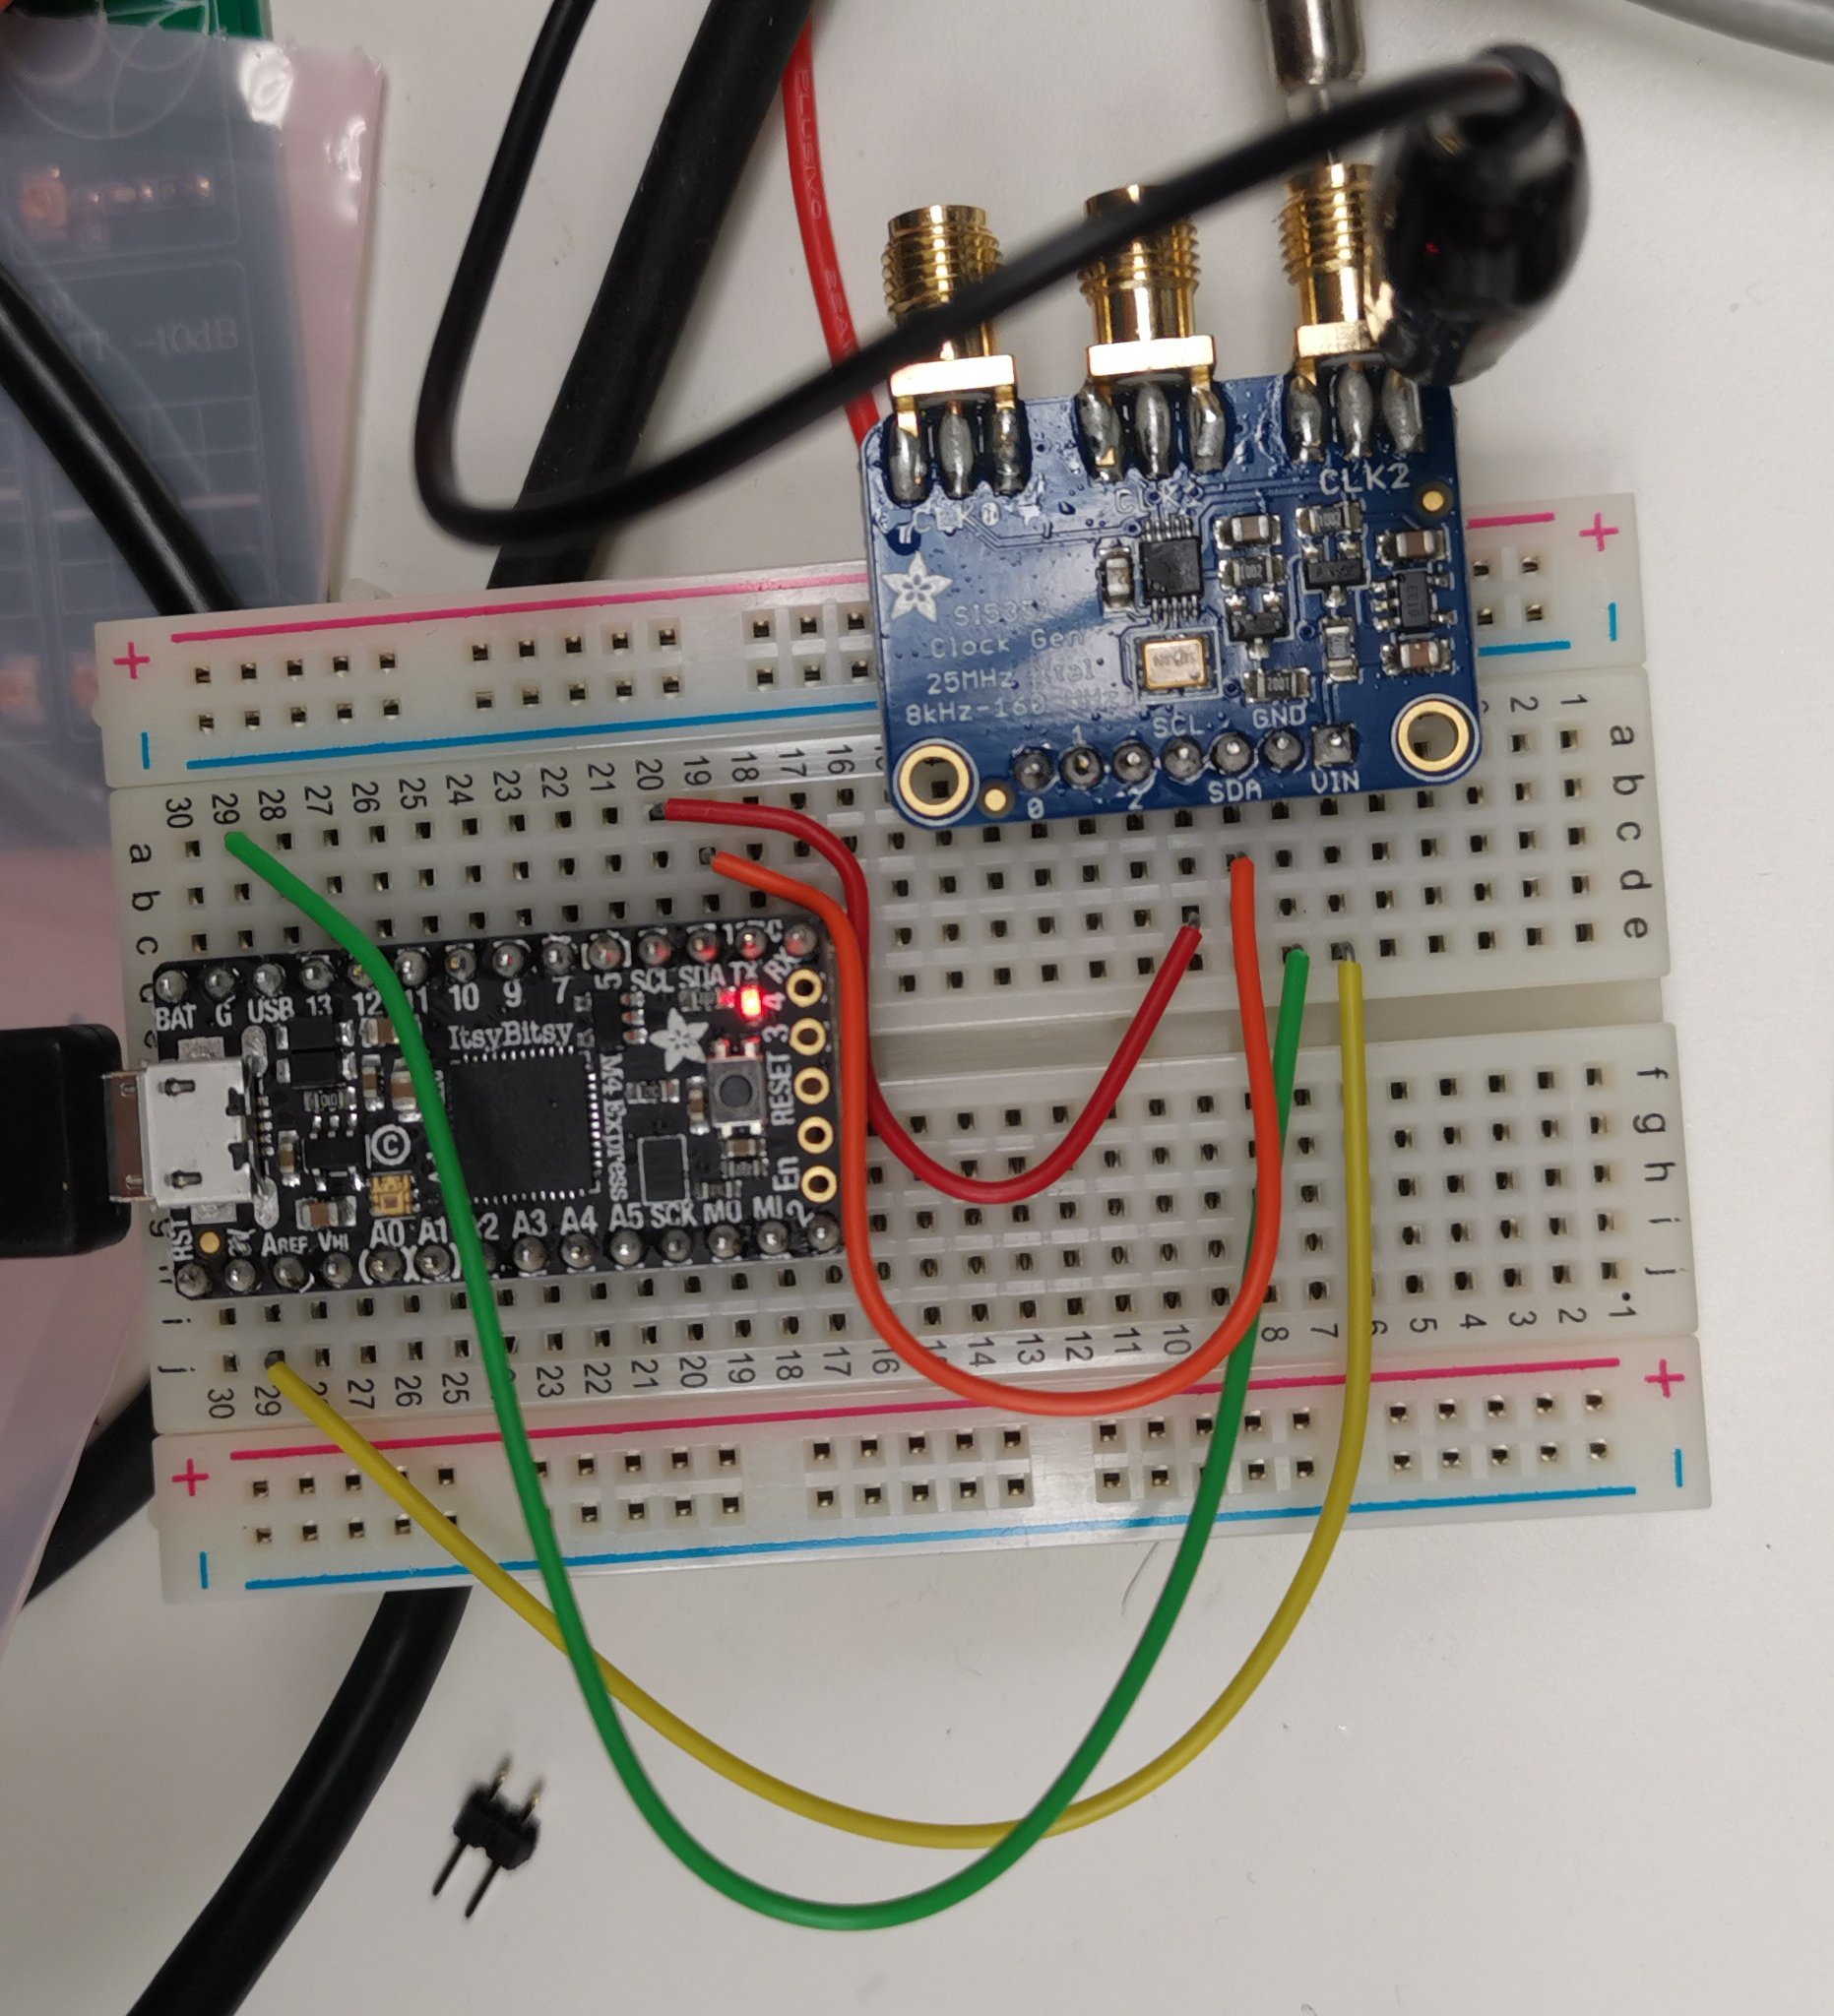
\includegraphics[width=.4\linewidth]{./pics/itsybitsy_si5351.jpg}
    \caption{Si5351 Clock Generator controlled By ItsyBitsy}
    \label{fig:assembly}
\end{figure}

The assembled circuit is shown in \Cref{fig:assembly}.

\section{Results}

We generated three different signals at 10.706KHz (\Cref{fig:clock_10_70k}), 13.5531MHz (\Cref{fig:clock_13_55m}), and 112.5MHz (\Cref{fig:clock_112_5m}).
The generated clock signals are shown in \Cref{fig:clock}.

\begin{figure}[h]
    \centering
    \begin{subfigure}{.33\linewidth}
        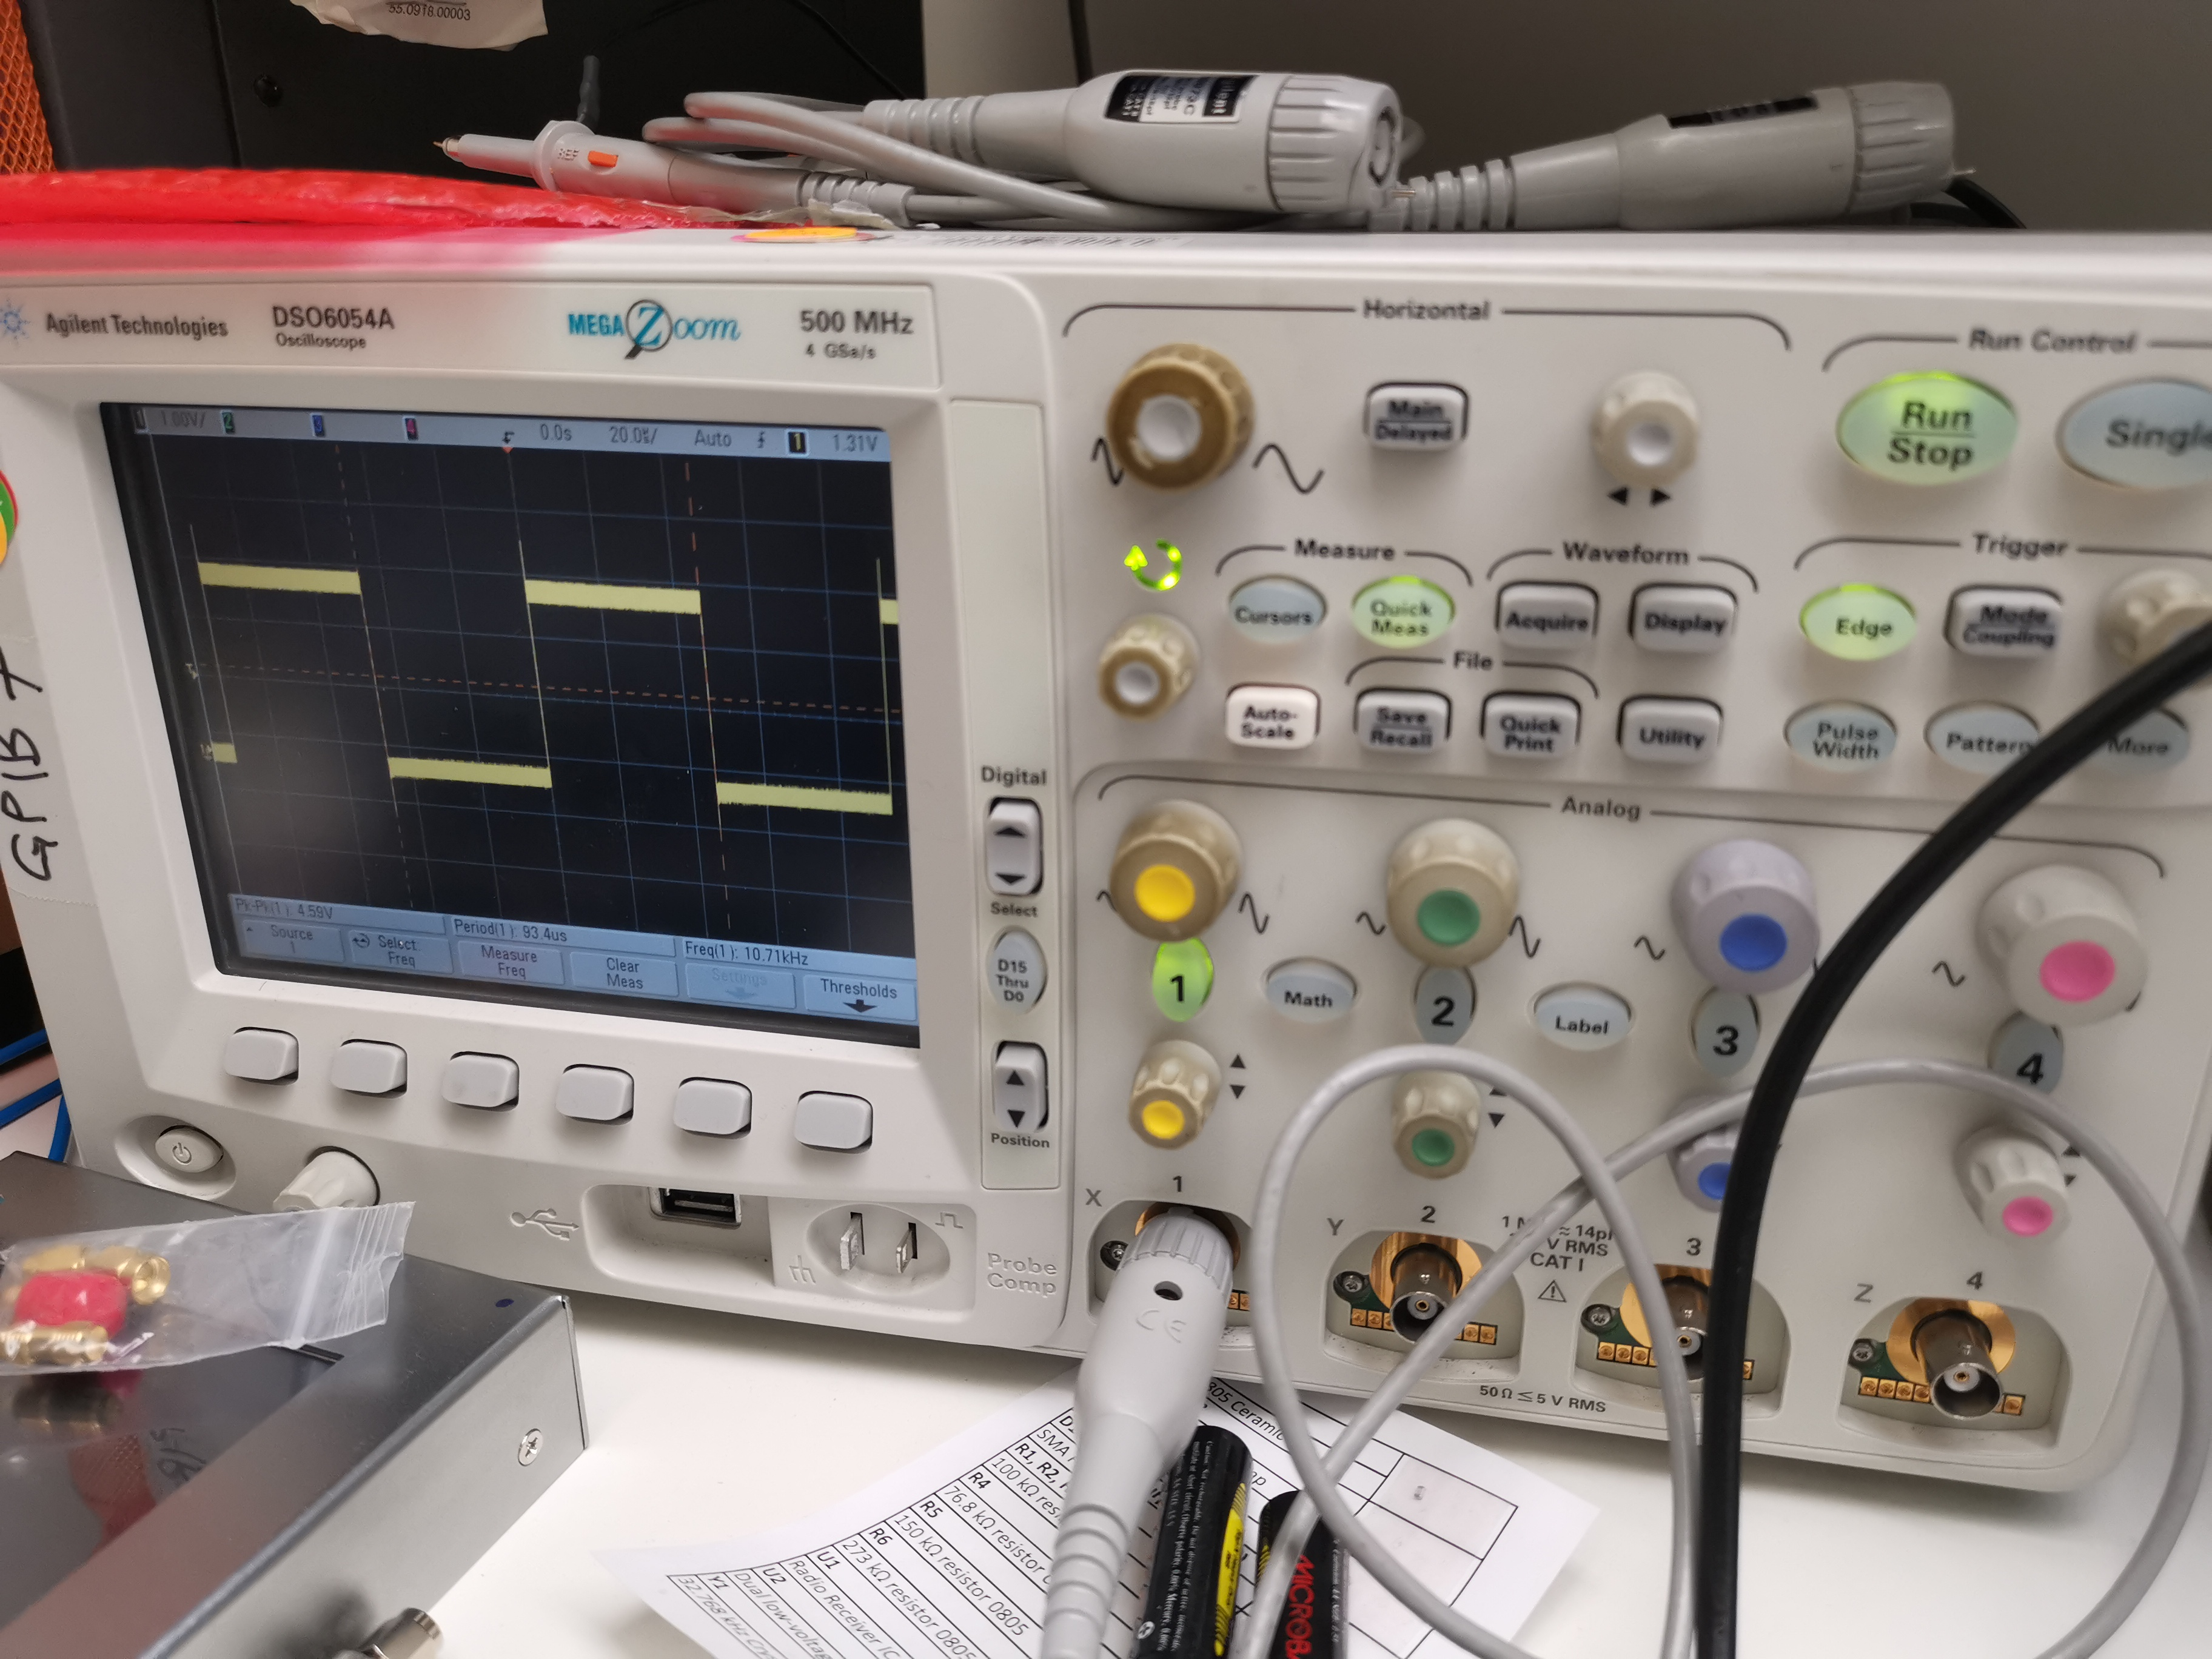
\includegraphics[width=.9\linewidth]{./pics/clock_10_70khz.jpg}
        \caption{10.706kHz generated clock signal}
        \label{fig:clock_10_70k}
    \end{subfigure}%
    \begin{subfigure}{.33\linewidth}
        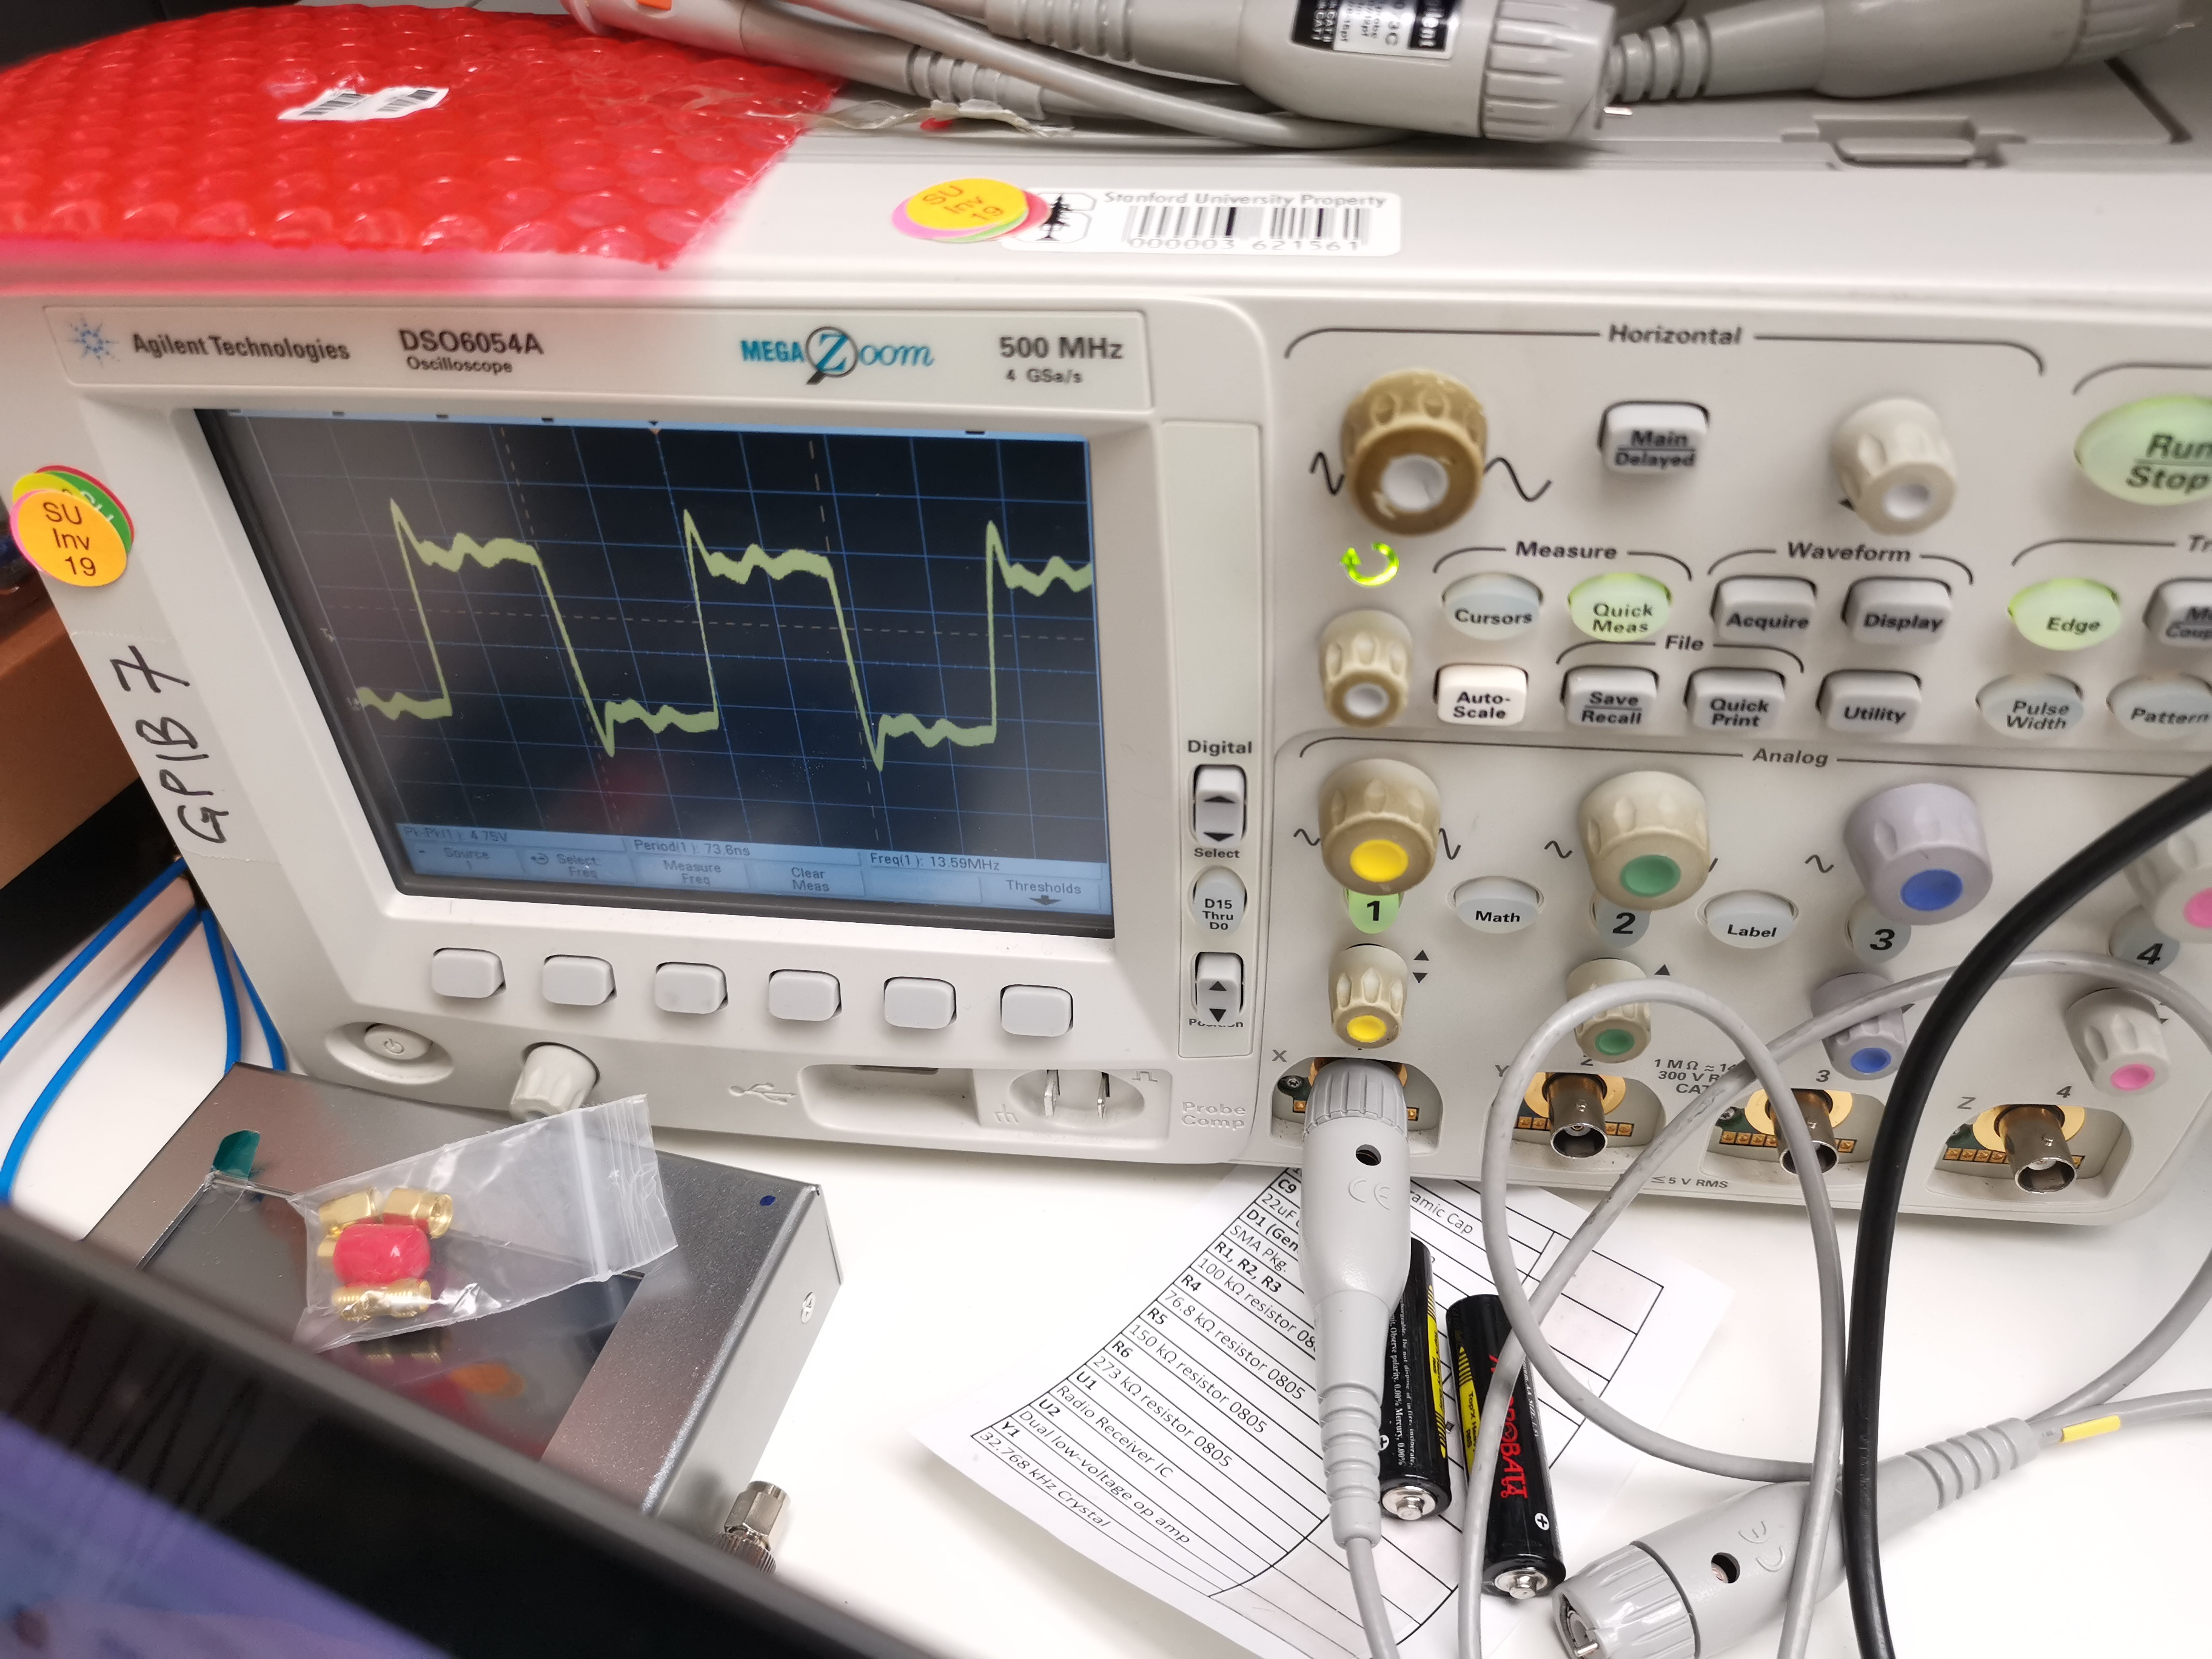
\includegraphics[width=.9\linewidth]{./pics/clock_13_55mhz.jpg}
        \caption{13.5531MHz generated clock signal}
        \label{fig:clock_13_55m}
    \end{subfigure}%
    \begin{subfigure}{.33\linewidth}
        \includegraphics[width=.9\linewidth]{./pics/clock_112_5mhz.jpeg}
        \caption{112.5MHz generated clock signal}
        \label{fig:clock_112_5m}
    \end{subfigure}%
    \caption{Generated Clock Signals at Various Frequencies}
    \label{fig:clock}
\end{figure}

\section{Discussion}

\subsection{How are all these different frequencies generated?}
\label{sec:block_diagram}

The datasheet claims that the Si5351 can generate frequencies from 8 KHz to 160 MHz, a 20,000 times difference between the lowest frequency and the highest frequency.
In addition, the reference clock needed is only at 25MHz, more than six times lower than the highest generated frequency.
How is all this accomplished?

\begin{figure}[h]
    \centering
    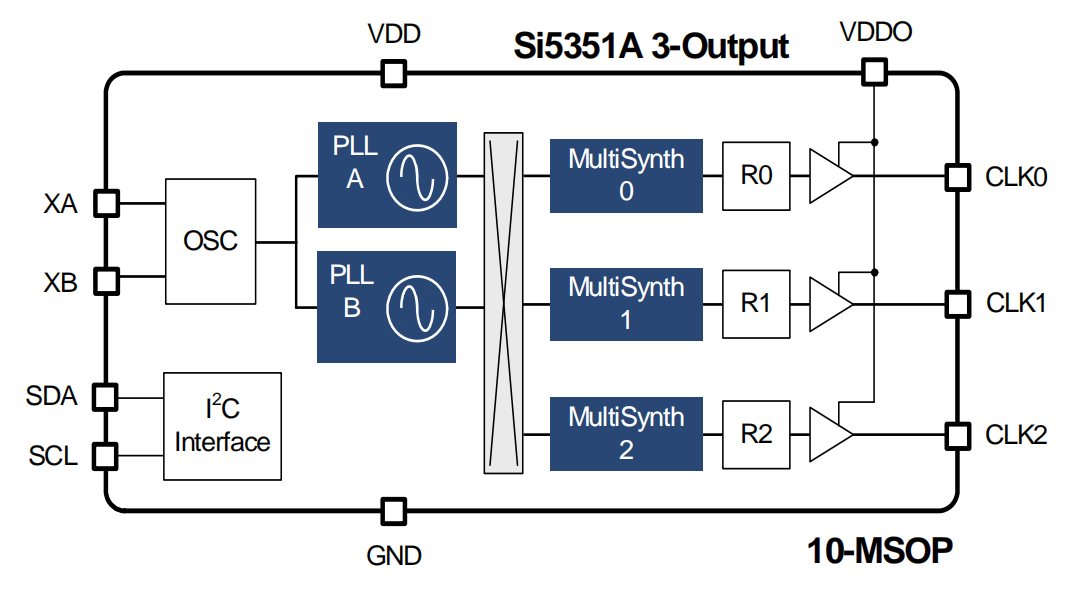
\includegraphics[width=.8\linewidth]{./pics/si5351a_block_diagram.png}
    \caption{Detailed Block Diagram of Si5351A 3-Output}
    \label{fig:si5351_block}
\end{figure}

The detailed block diagram of Si5351 is shown in \Cref{fig:si5351_block}.
As we can see, internally, the input clock is first multiplied to high intermediate frequencies PLL A and PLL B using phase lock loops.
This not only enables the IC to synthesize output frequencies higher than the input frequency, but also allows for better resolution in the output frequencies.
The phase lock loops support both integer and fractional multiples of the input clock frequency.
For our purposes, we configured PLL A to be 36 times the input clock (900MHz), and PLL B to be $24 \frac{2}{3}$ times the input clock (616.6667MHz).

Then, the higher intermediate frequencies are passed through high resolution MultiSynth fractional dividers, which can divide the intermediate frequency by either integers or fractions.
For our purposes, we configured clock 0 to be PLL A divided by 8 (112.5MHz = 900MHz / 8), clock 1 to be PLL B divided by $45\frac{1}{2}$ (13.5531MHz=616.6667MHz / 45.5).

Finally, an ouput R divider can divide the frequency further by $2^k, k\in\{0,...,7\}$, to get frequencies as low as 8 kHz.
For our purposes, to obtain clock 2, we first used the MultiSynth to divide PLL B by 900, and then applied an additional R divider of 64 (10.706KHz = 616.6667MHz / 900 / 64).

In conclusion, by having one frequency-multiple stage and two frequency-divide stages, the Si5351 is able to generate three non-integer related output frequencies from 8KHz to 160MHz.

\subsection{Why do the waveforms in for different frequencies look so different?}
\label{sec:waveform_diff}

As we can see in \Cref{fig:clock}, the output for 10.7KHz (\Cref{fig:clock_10_70k}) looks very much like a square wave, the output for 13.5MHz (\Cref{fig:clock_13_55m}) has some ripples, while the output for 112.5MHz (\Cref{fig:clock_112_5m}) doesn't resemble a square wave at all.

This shows that as frequency goes up, the output waveforms are more ``smoothed'' from the ideal square wave.
Mathematically, smoothing in the time domain just corresponds to low-passing in the frequency domain.
This is reasonable to expect, as all circuits have some capacitive parasitics, which can effectively act as low-pass filters at high-enough frequencies.

\subsection{Quadrature Signals}
\label{sec:iq}
Conveniently, the Si5351 offers configurable initial phase offset for all clock outputs.
This means that for certain frequencies, we can connect two output clocks to the same PLL, and set their time delays to be different by exactly 1/4 the output period to generate a pair of I and Q clock signals.

However, this doesn't work for all output frequencies.
The initial phase offset is specified as a 7-bit unsigned integer with one LSB equivalent to a time delay of Tvco/4, where Tvco is the period of the VCO/PLL associated with the output.
This means that to get an output phase difference of exactly 90 degrees, the output frequency cannot be less than $1/2^7=1/128$ of the PLL.
In addition, if we use fractional frequency division in the MultiSynth dividers, we may not be able to get exactly 90 degrees difference at the output.

\section{Conclusions}
In this lab, we demonstrated that a clock generator IC is easy to use and can generate a wide range of different output frequencies.
We explored the implementation of Si5351 (\Cref{sec:block_diagram}), why the output waveforms are different at different frequencies (\Cref{sec:waveform_diff}), and potential use of the IC to generate IQ signals (\Cref{sec:iq}).
This work can be extended by better understanding the limitations of the Si5351 IC, as well as exploring other potential applications.

\end{document}